\documentclass[11pt,a4paper]{report}

\usepackage[english]{babel} 
\usepackage[utf8]{inputenc} % Unicode
\usepackage{graphicx} 
\usepackage{url} 
\usepackage{amsmath}
\usepackage{textcomp} 
\usepackage{lipsum}
\usepackage{multirow} 
\usepackage[pdftex,hidelinks]{hyperref}
\usepackage{listings}
\usepackage{natbib}
\usepackage{float}% If comment this, figure moves to Page 2
\usepackage{graphicx}
\usepackage{hyperref}
\usepackage{verbatim}
\usepackage{textcomp}
\usepackage{caption}
\usepackage{subcaption}
\usepackage{acronym}
\usepackage{blindtext}
%%%%%%%%%%%%%% Referências
\makeatletter
\def\thebibliography#1{\chapter*{REFERENCES\@mkboth
{REFERENCES}{REFERENCES}}\list
{[\arabic{enumi}]}{\settowidth\labelwidth{[#1]}\leftmargin\labelwidth
\advance\leftmargin\labelsep
\usecounter{enumi}}
\def\newblock{\hskip .11em plus .33em minus .07em}
\sloppy\clubpenalty4000\widowpenalty4000
\sfcode`\.=1000\relax}
\makeatother
%%%%%%%%%%%%%

\def\R{{\textsl{R }}}
\def\Shiny{\textsl{Shiny }}
\def\sar{\textsl{SARS-CoV-2 }}


\title{A \Shiny application for visualising SARS-CoV-2 vaccination coverage in Portugal}

\author{
  Bruna Araújo\\
  \texttt{A84408}
  \and
  Matias Capitão\\
  \texttt{A82726} \\ 
  \\ Supervisor:\\
  Cecília Castro\\
  \and
  Rafael Antunes\\
  \texttt{A77457}
}
\date{}

\linespread{1.5}

\begin{document}

\maketitle

\begin{abstract}
    For this project, was proposed to us the development of an application with the theme: “Development of a Shiny application to visualize data on the SARS-CoV-2 epidemic”.
    
    
    The main objective was to develop a Shiny application for visualization
    of data and analysis of various indicators that allow, in an interactive way, the monitoring of the
    SARS-CoV-2 epidemic in Portugal. \\
    This project had two phases: the first one was a phase to study the data and workflow of an R Shiny application, and the second phase was the phase of implementation.\\
    We end up to publish our application in \textit{Shinyapps.io} that is an online service for hosting Shiny apps in the cloud.
    
    
     
    






    

    
    
    

\end{abstract}

\tableofcontents
\newpage

\listoffigures
\newpage

\newpage

{\huge\textbf{Acronym List}}\\
\begin{acronym}[MPC] % Give the longest label here so that the list is nicely aligned
\acro{IDE}{Integrated Development Environment}
\acro{WHO}{World Healh Organization}
\acro{EU}{European Union}
\acro{ECDC}{European Centre for Disease Prevention and Control}

\end{acronym}


\chapter{Introduction}
In the context of the UC “Project” of the Degree in Computer Science, it was proposed to us the development of a Shiny application that would allow the visualization of variables associated with the COVID-19 pandemic in Portugal, as well as in its different regions. Once the vaccination process is ongoing and is in the order of the day, the application focuses on this process. 
This report is organized essentially in two main  parts. Firstly is presented an introduction with a briefly reference to R, RStudio and the Shiny package. Also we  contextualize the theme, namely in what concerns to the disease and the vaccination process in Portugal.
In the second part of this report, Chapter 2, we began by presenting the data,  its structure and features. Next is made a detailed description of the functionalities of the app, referring to the main attributes and properties of the Shiny apps that allow the development and application of the app developed in this work, presenting several examples of  implemented functions.

\section{The \R Program and \Shiny package}

\textbf{\R}  is a program created in 1993 by Ross Ihaka and Robert Gentleman  defined as
"a language and environment for statistical computing and graphics" \cite{R-project website}.
\\
 RStudio is an integrated development environment (IDE) for R. \cite{rstudio}
\begin{figure}
\centering
\begin{subfigure}{.5\textwidth}
  \centering
  
\includegraphics[width=3cm]{images/R.jpg}
  \label{fig:sub1}
\end{subfigure}%
\begin{subfigure}{.5\textwidth}
  \centering
  
\includegraphics[width=5cm]{images/Rstudio.png}
  \label{fig:sub2}
\end{subfigure}
\caption{Logos of R and RStudio}
\label{fig:test}
\end{figure}
\\
R has over 10,000 packages in the CRAN repository which are constantly growing. 
\textbf{\Shiny} is an \R package that makes easy to build interactive web applications \cite{shiny} .
\\
With this package we can combine the computational power of \R with the versatility and interactivity of modern web. This feature it's relevant to develop plots and graphics that can be understood by everyone, and looking pretty while doing it.




\section{COVID-19 pandemic}
%\subsection{Brief description}



\sar is the name of the coronavirus that caused the current COVID-19 pandemic. According to \ac{WHO}, the first human cases of COVID-19, were first reported from Wuhan City, China, in December 2019. 
The main symptoms of Covid-19 are fever, cough, breathing difficulties, loss of smell and taste. 
It's a disease that attacks all age levels and is transmitted mainly by air, via particles that we expel. \\
There are several reasons for the pandemic to spread globally, mainly the fact that a patient may be asymptomatic, which can cause him to transmit the virus without knowing it. For the same reason, the fact that the incubation period is about 14 days is also a factor to be taken into account. 

\subsection{Vaccination}
Vaccines are substances made up of pathogens (viruses or bacteria), living or dead, or their derivatives. They stimulate the immune system to produce antibodies that act against pathogens that cause infections.

Vaccination is a way to protect people from harmful diseases. It uses the body's natural defenses to build resistance to specific infections and makes the
 stronger immune system.
It reduces the possibility of contracting the disease and thus prevents it from spreading.
\\
As soon as the COVID-19 pandemic took hold in the world, research for the production of safe and effective vaccines began immediately. Vaccination is critical to ending the COVID-19 pandemic. WHO is working tirelessly with partners to develop, manufacture and distribute safe and effective vaccines.
\\
Until May 10, 13 vaccines have been authorized by at least one national regulatory authority for public use. However, in Europe, after consulting the list of authorized vaccines on the \cite {EU} official website of the \ac{EU}, we have four vaccines available: 
\begin{itemize}
    \item BioNTech-Pfizer - (2020/12/21)
    \item Moderna - (2021/01/06)
    \item AstraZeneca - (2021/01/29)
    \item Johnson \& Johnson - (2021/03/11)
\end{itemize}
But it's not the vaccines that will stop the pandemic, it's the vaccination. 
\\





\section{Portugal}

\subsection{Brief description}
Portugal is a country in Europe with a resident population of around 10.2 million inhabitants.  \\
According to the local statistics institute, INE (Instituto Nacional de Estatística - National Statistics Institute), in the publication dated 2019 and edited in 2020, called \cite{pubINE}"Demographic Statistics - 2019", we can find some interesting information such as:
\begin{itemize}
    \item In percentage terms, relative to \textbf{sex},
    \begin{itemize}
        \item \textbf{47,2\textdiscount} of the population is \textbf{male};
        \item \textbf{52,8 \textdiscount} of the population is \textbf{female}.
    \end{itemize}  
    \item In terms of \textbf{age} percentages, 
    \begin{itemize}
        \item \textbf{13,6\textdiscount} of \textbf{young people} (0-14 y/o);
        \item \textbf{64.3\textdiscount} of people of \textbf{working age} (15-64 y/o);
        \item \textbf{22.1\textdiscount} of \textbf{elderly people} (65+ y/o). 
    \end{itemize}
\end{itemize}

Se calhar por aqui alguns graficos relativos ao descrito acima nao é má ideia.

\subsection{Regions}
In terms of NUTS II regions, Portugal is divided in seven groups.
The structuring of the Portuguese territory according to the New Territorial Units for Statistical Purposes, NUTS 2013,  in application in the National Statistical System since 1 January 2015 is composed of seven NUTS II: North, Centre, Lisbon Metropolitan Area (AML), Alentejo and Algarve regions, on the mainland, and the two autonomous regions. \cite{INEE}
\begin{figure}[h]
\centering % para centralizarmos a figura
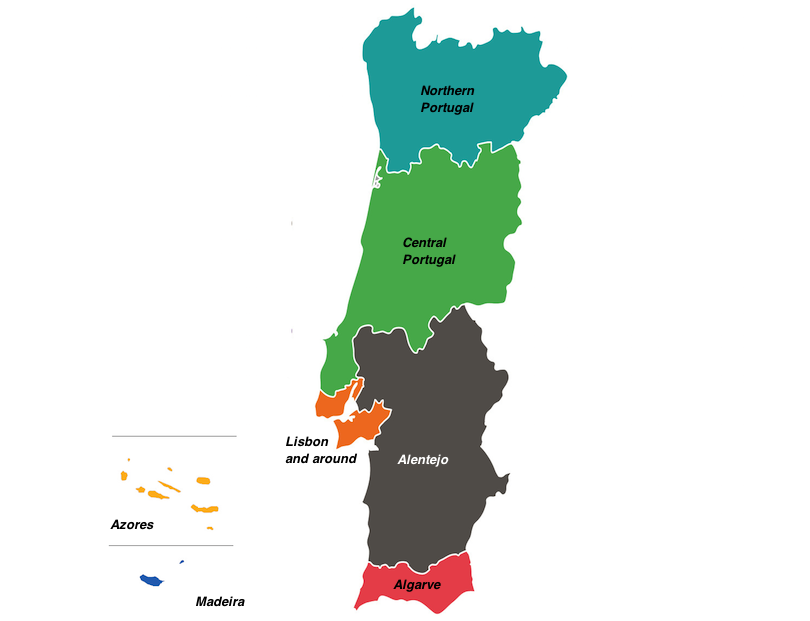
\includegraphics[width=10cm]{images/portugal.png} 

\caption{Portugal's Regions}
\label{figura:qualquernome}
\end{figure}

We'll describing them below, also mentioning some statistical data that may be interesting. \\
All information related to the labor market in the regions was obtained by consulting the  website of the European Commission \cite{trab}. The demographic percentages presented are based on data from  National Institute of Statistics of Portugal, INE. 

\subsubsection{North}
The employment structure in the North region presents 3 sub-regions with specific characteristics: 
The Porto Metropolitan Area, with a strong incidence of services (mainly trade) with greater technological and knowledge intensity. A surrounding shore, where industrial employment is  higher than the national average and rural areas, where nearly half of employment is concentrated in agriculture or non-commercial services.

In terms of {\textbf{demographics}}:
    \begin{itemize}
        \item Population density: {34,73\textdiscount} . 
        \item Gender: {47,2\textdiscount} male and {52,8\textdiscount} female.
        \item Age: 
        \begin{itemize}
        \item {12,63 \textdiscount} aged 14 and younger;
        \item {66,43\textdiscount} aged 15 to 64;
        \item {20,94\textdiscount} aged 65 and older.
        \end{itemize}
    \end{itemize}

\subsubsection{Center}
In this region, the Services sector is the most relevant in terms of employment - with emphasis on Trade and Vehicle Repair, Health and Social Support Services and the Education. \\
In terms of {\textbf{demographics}}:
    \begin{itemize}
        \item Population density: {21,54\textdiscount} . 
        \item Gender: {47,42\textdiscount} male and {52,58\textdiscount} female.
        \item Age: 
        \begin{itemize}
        \item {12,05 \textdiscount} aged 14 and younger;
        \item {63,42\textdiscount} aged 15 to 64;
        \item {24,53\textdiscount} aged 65 and older.
        \end{itemize}
    \end{itemize}
    
\subsubsection{Metropolitan area of Lisbon }
This is the region with the highest population density in the country. It's the region with the highest concentration of services, with emphasis on services provided mostly by the Public Sector; Education; Health and social support services.\\
In terms of {\textbf{demographics}}:
    \begin{itemize}
        \item Population density: {27,81\textdiscount} . 
        \item Gender: {46,71\textdiscount} male and {53,29\textdiscount} female.
        \item Age: 
        \begin{itemize}
        \item {15,88\textdiscount} aged 14 and younger;
        \item {62,04\textdiscount} aged 15 to 64;
        \item {22,08\textdiscount} aged 65 and older.
        \end{itemize}
    \end{itemize}
    
\subsubsection{Alentejo}
This is the region with the lowest population density in the country. Most of the region's territory is dedicated to Agriculture, allied to cattle breeding and also forestry.\\
In terms of {\textbf{demographics}}:

    \begin{itemize}
        \item Population density: {6,84\textdiscount} . 
        \item Gender: {47,97\textdiscount} male and {52,03\textdiscount} female.
        \item Age: 
        \begin{itemize}
        \item {12,4\textdiscount} aged 14 and younger;
        \item {62,05\textdiscount} aged 15 to 64;
        \item {25,55\textdiscount} aged 65 and older.
        \end{itemize}
    \end{itemize}
    
\subsubsection{Algarve}
The economic structure of this region is based on 5 strategic sectors associated with the region's natural resources: hospitality, catering and tourism, health, creative activities, agri-food and maritime activities. 
In terms of {\textbf{demographics}}:
    \begin{itemize}
        \item Population density: {34,73\textdiscount} . 
        \item Gender: {47,2\textdiscount} male and {52,8\textdiscount} female.
        \item Age: 
        \begin{itemize}
        \item {12,63\textdiscount} aged 14 and younger;
        \item {66,43\textdiscount} aged 15 to 64;
        \item {20,94\textdiscount} aged 65 and older.
        \end{itemize}
    \end{itemize}
    
\subsubsection{Azores autonomous region}
The region's economy is fundamentally based on activities mainly from the Public Sector (Public Administration, Social Security, Education, Health and Social Support activities). The activities of Trade and Repair of Vehicles and Accommodation and Restoration are equally important in employment in the region. \\
In terms of {\textbf{demographics}}:
    \begin{itemize}
        \item Population density: {2,36\textdiscount} . 
        \item Gender: {48,55\textdiscount} male and {51,45\textdiscount} female.
        \item Age: 
        \begin{itemize}
        \item {15,37\textdiscount} aged 14 and younger;
        \item {69,69\textdiscount} aged 15 to 64;
        \item {14,99\textdiscount} aged 65 and older.
        \end{itemize}
    \end{itemize}
    
\subsubsection{Madeira autonomous region }
In terms of more established work areas, this region is very similar to the Azores region. Tourism has an important role for both regions.\\
In terms of {\textbf{demographics}}:
    \begin{itemize}
        \item Population density: {2,47\textdiscount} . 
        \item Gender: {46,67\textdiscount} male and {53,33\textdiscount} female.
        \item Age: 
        \begin{itemize}
        \item {13,11\textdiscount} aged 14 and younger;
        \item {69,91\textdiscount} aged 15 to 64;
        \item {16,98\textdiscount} aged 65 and older.
        \end{itemize}
    \end{itemize}









\section{COVID-19 and Vaccination in Portugal}

%\subsection{Brief description}

%SARS-CoV-2 (Severe Acute Respiratory Syndrome coronavirus) is a new type of coronavirus that causes a respiratory disease called coronavirus disease 19, know as COVID-19. It was first detected in December 2019 has quickly spread globally.

Portugal recorded the first confirmed case of COVID-19 on March 2 and the first death occurred
on March 16. Since then we have added more than 800 thousand registered cases and more than 16 thousand deaths.

Portugal was severely affected by COVID-19, being considered, in the middle of January 2021, as the worst country in the world in terms of infection and mortality rates per million inhabitants and the worst country in Europe with the highest average of cases COVID-19 daily reports, with Portugal reaching a maximum of 16432 cases and 303 deaths on 28 January 2020.

\subsection{Vaccination}

   To end this pandemic, a large part of the world needed to be immune to the virus. The safest way to achieve this was through a vaccine, so with the help of investments by companies, governments, international health organizations and university research groups it was possible to develop a series of vaccines including Phyzer, Moderna, Astrazeneca, Johnson & Johnson, among others.

   The first vaccine administered in Portugal was on December 27, 2020. The first vaccine was António Sarmento, 65, director of the Infectious Diseases Service, at Hospital de São João, in Porto and since then more than 2 million doses of vaccine have been administered. Despite the fact that the entire Portuguese population has access to a vaccine, depending on their clear clinical condition, Portugal opted for a vaccination plan divided into 3 phases, that is, priority groups were defined, as they are more vulnerable to COVID-19, as an example health professionals, professionals and residents of residential structures for the elderly and similar institutions, who were part of the first vaccination phase.






\chapter{The Shiny App}

\section{Data :: Structure and Features}
The data that we used to develop this application was downloaded from the \ac{ECDC} which is an \ac{EU} agency aimed at strengthening Europe's defenses against infectious diseases.
\\
As we can read in the \ac{ECDC} website \cite{dataDownload}, they are providing an overview of the progress in the rollout of COVID-19 vaccines in adults across \ac{EU} countries.
\begin{figure}[h]
\centering % para centralizarmos a figura

\includegraphics[width=3cm]{images/ecdc.png} 

\caption{ECDC logo}
\label{figura:qualquernome}
\end{figure}

The data is collected through The European Surveillance System (TESSy) and they publish the updated data, every week on Thursdays. In Portugal, the entity responsible to send the data is the Ministry of Health.

\subsection{Structure of the data}
The dataset  downloaded in each interaction with the app in format \verb!csv!, has the following columns:

\begin{itemize}
    \item \textbf{YearWeekISO} - Date information in weeks:  week number and year;
    \item \textbf{FirstDose} - Number of first dose vaccine administered to individuals during the reporting week;
    \item \textbf{FirstDoseRefused} - Number of individuals refusing the first vaccine dose;
    \item \textbf{SecondDose} - Number of second dose vaccine administered to individuals during the reporting week;
    \item \textbf{UnknownDose} - Number of doses administered during the reporting week where the type of dose was not specified;
    \item \textbf{NumberDosesReceived} - Number of vaccine doses distributed by the manufacturers to the country during the reporting week;
    \item \textbf{Region} -  Region of the Reporting Country.
   
    In order to know the region to which these codes relate to, it was necessary another excel document. This document also brought another important component, namely, the population of each region. Having said this:
    \begin{itemize}
        \item PTCSR01 - Alentejo; Population - 466 690
        \item PTCSR02 - Algarve; Population - 438 406
        \item PTCSR03 - Autonomous Region of Azores ; Population - 242 796
        \item PTCSR04 - Centre; Population - 1 650 394
        \item PTCSR05 - Metropolitan Area of Lisbon; Population - 3 674 534
        \item PTCSR06 - Autonomous Region of Madeira; Population - 254 254
        \item PTCSR07 - North; Population - 3 568 835

    \end{itemize}
    \item \textbf{Population} - Age-specific population for the country (unfortunately, in Portugal, this hasn't been exactly right, it only has the total population of Portugal);
    \item \textbf{ReportingCountry} - The country that is providing the information;
    \item \textbf{TargetGroup} - Target group for vaccination;
    \item \textbf{Vaccine} - Name of vaccine;
    \item \textbf{Denominator} - Population denominators for target groups.

We will show next, a little example of the dataset already filtered for Portugal.

\end{itemize}

\begin{figure}[h]
\centering % para centralizarmos a figura
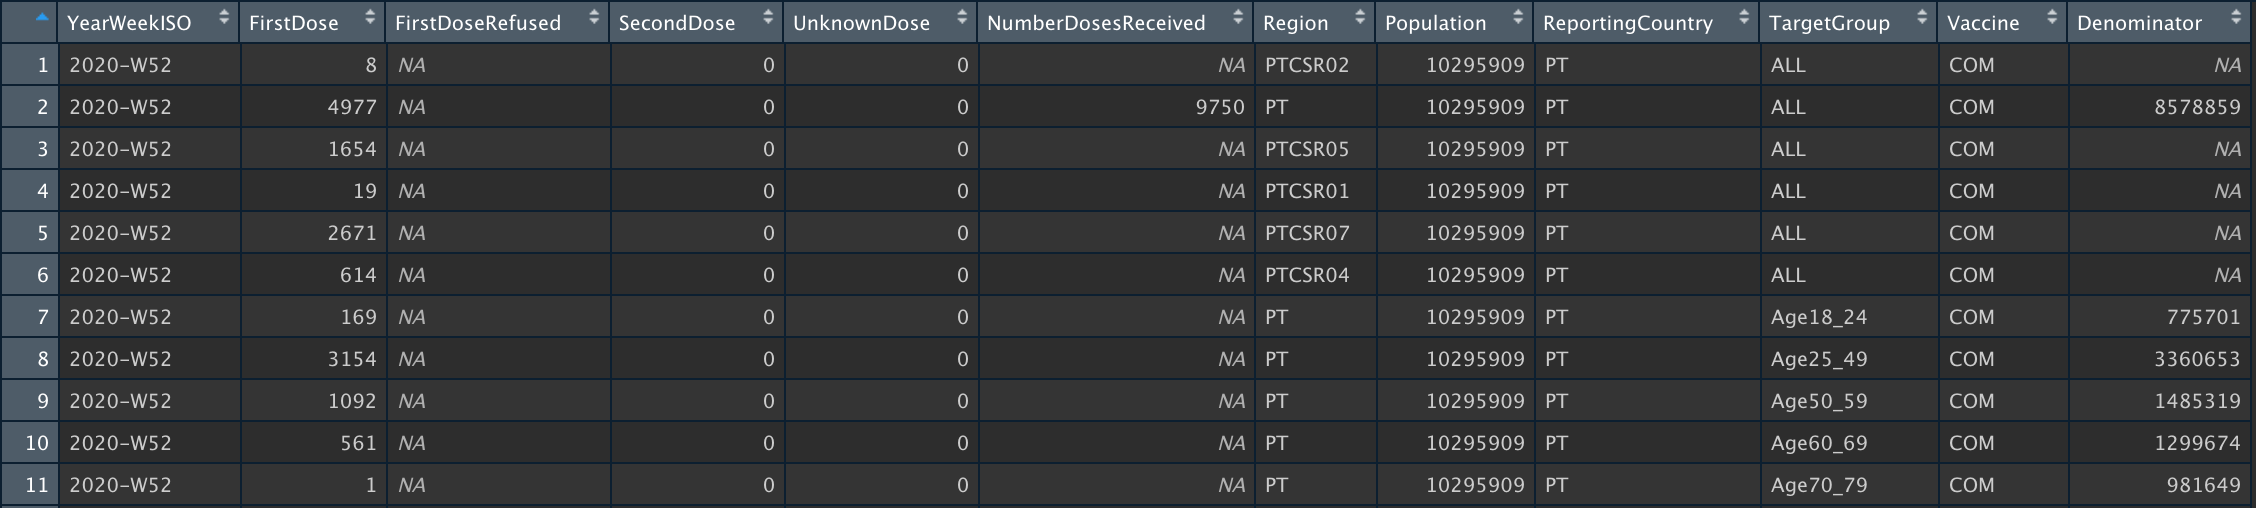
\includegraphics[width=15cm]{images/dataset.png} 

\caption{Excerpt from the dataset }
\label{figura:qualquernome}
\end{figure}





\section{Development}
The R Shiny framework is an RStudio package that makes it incredibly easy to build interactive web applications with R. A Shiny has the benefit of allowing us to create highly effective reports and data visualizations where the user can explore a set of data.

Shiny apps are divided into two parts: 

\begin{itemize}
    \item server.r
    \item ui.r (UI)
    
\end{itemize}
 % se tiver a der merd* corrijam 
 
The ui specification defines:
\begin{itemize}
    \item  Layout functions to configure the visual structure of the html page that will be generated when the application is executed. The fluidPage() function embeds and configures all the necessary and sufficient HTML, CSS and JavaScript code for the application. To create more complex layouts, you need to call layout functions inside fluidPage().
    \item Input control functions that will allow the user to interact with the application. Functions such as sliderInput(), selectInput(), textInput(), numericInput() can be used. All these functions have inputID as their first argument, simple string, with the same restrictions as the object names of R, and unique. This identifier is used to bind the ui to the server.
    If in the ui the inputID = “name”, the server will access it using input?name. The second argument, label, is also important as it contains the text that appears in the application's layout.
    \item Output controls that indicate where to place output with reactive behavior. Examples of output control functions are textOutput(), tableOutput(), among others. As with input control functions, the first argument must be the unique ID. If, for example, in the ui an ID with the name “plot” is defined, on the server the access is output$plot.



 In the server specification, functions that allow calculations to be performed and updated (using reactivity) are implemented. The server controls what data will be through the UI. The server will be where you upload and collate the data and then set your options (ie graphics) using input from the UI.
 
 
 For this purpose, specific rendering functions (render functions) are used. Each render{Type} function produces a specific type of output (for example, renderTable() produces tables, renderText() produces text). Usually these functions are paired with {Type}Output functions (for example renderTable() because it is paired with tableOutput()).


 
 Even though we created two separate files for our application, namely server.r and ui.r , shiny supports single file applications. A single file configuration puts both the server and user interface code in a single app.R file, whereas the multiple file configuration puts them in their own separate files. Functionally, these configurations will produce the same app. The multiple file configuration is generally preferred, especially for larger applications, as it usually makes code easier to manage. For smaller apps, the single file configuration is likely a more efficient way to go.


\subsection{Reactivity in shiny}
Like in other web applications, in Shiny, you express server logic using reactive programming.
\\
The main idea of reactive programming is to specify the dependency graph so that when an input is changed, all related outputs are also updated. 
%for example, we don't need to tell an output to update because due to reactivity, the information is always updated. automatic, making the flow of an application considerably simpler.
\\
Reactivity is what makes applications responsive. Allows the application to update itself instantly whenever the user interacts with the application, requesting any visualization, with updated data.
\\
In Shiny, reactivity creates the illusion that changes to input values automatically flow to the outputs -- graphics, text, and tables that use the input --  and cause them to update. This flow behavior (such as current in a river or electricity) that pushes information from input to output is not real. In fact, in R an expression is only updated when it is executed (lazy evaluation).
\\
So, the idea is: the server re-execute the instructions very frequently, so it knows the input change very quickly, and acts as if it were bound to the input or as if input pushed its new value to the output.
\\
This is the approach that Shiny uses to create reactivity. This is why session R is busy when starting a Shiny application (for example, it is not possible to use the R console when the application is running). The server is using session R to monitor the application and rerun the expressions.
\\
However, Shiny takes this approach a step further, creating an alert system that lets you know exactly what expressions need to be rerun.
\\
Thus, although the server still checks the application at regular intervals (of microseconds), instead of rerunning each expression, it only executes the expressions that the alert system flagged as out of date. If alerts appear, the server executes all expressions that are out of date at the time - this event is called flush and is the key to reactivity as it allows the server to update the application as quickly as possible, appearing to flow instantly from inputs to outputs.
\\
We can see several examples of the use of reactivity in the code of our app. For example, in \verb!UI! (\ref{ui}) and in \verb!server! (\ref{server})
\begin{figure}[h]
\centering % para centralizarmos a figura
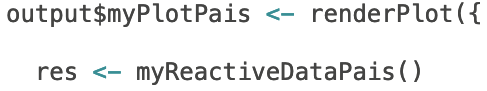
\includegraphics[width=150px]{images/reatividadeUI.png} 
\caption{reactivity:: UI}
\label{ui}
\end{figure}
\begin{figure}[h]
\centering % para centralizarmos a figura
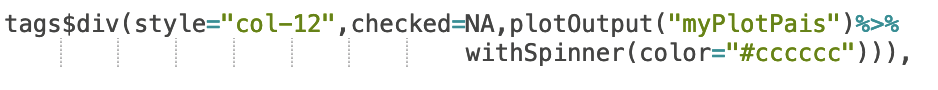
\includegraphics[width=250px]{images/reatividadeSERVER.png} 
\caption{reactivity:: server}
\label{server}
\end{figure}
%In our app we use reactive functions, as it is a way to control which parts of the app are updated, avoiding unnecessary calculations that can slow down your app.

%In our application we use reactive functions as it is a way to control which parts of the application are updated, avoiding unnecessary calculations that can make your application slow.



%\begin{figure}[h]
%\centering % para centralizarmos a figura
%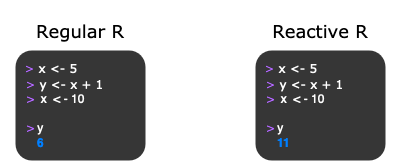
\includegraphics[width=7cm]{images/react.png} 

%\caption{Example of Regular R - Reactive R}
%\label{figura:qualquernome}
%\end{figure}




%For example, in our app //PUT AN EXAMPLE OF OUR APP


%\subsection{Render functions}

%The main function for generating documents in R Markdown, from the rmarkdown package, is a render ().
%The render () function is a wrapper that internally calls knitr :: knit () and later converts the document to .html using Pandoc, which is a document and open source converter.Uma função render que usamos na aplicação foi a renderPlot().

%To display the graphics in our application we use the renderPlot () tool. RenderPlot is a reactive function that can take input data from the ui.R script and feed it into the server.R script. It then actively updates the information within its role.



\subsection{Data visualization}
Data visualization through maps, tables or graphs allows contextualizing and understanding information in a natural and efficient way.


R has libraries that allow us to get high quality graphics. In this report we mainly use \verb!ggplot2!, based on its own graphics grammar,  where the graphical representations are obtained by superimposing several stacking levels, allowing great flexibility in the construction of the graphics (Hadley Wickham, 2005).  \cite{ggplot2}
\\
Layers consist on the data (data.frame format), aesthetic attributes (data mapping definition), geometric objects (visual elements), facets (\verb!facets()!) functions that allow the execution of multiple graphics related to segments of data defined by factors), statistical transformations, coordinates (space where data is represented) and theme (\verb!theme()!, functions allow changing individual components of a theme).

\section{Implementation}

\subsection{User Interface}
In terms of \verb!User Interface!, it's pretty simple to implement an application with a good and intuitive layout. In our application, we have two main structures that were chosen, not only because, in our opinion, it's prettier, but also to show some different ways to see information. Our two structures are the followed: \\

\begin{figure}[H]
\centering
\includegraphics[width=300pt,trim=10 0 0 -10mm]{images/coiso.png}
\caption{Structures overview}
\label{fig:overview}
\end{figure}

We named the structures as \textit{'X'} and \textit{'Y'}, merely to be easier to see and explain the differences between them.\\
As we can see, both layouts have something in common: \\
\begin{itemize}
    \item \textbf{A} it's our navigation bar, commonly used in a lot of websites and web applications;
    \item \textbf{B} it's an area made by us with a few of \verb!CSS! that will show some relevant information of the data;
    \item \textbf{D} it's the area where all the data and information will appear.  
\end{itemize}

In the \verb!Structure 'X'!, the area \textbf{C} represents an area where the user can select the plot/s that want to display. It's possible to display more than one plot at the same time. \\ 
In the \verb!Structure 'Y'!, coming from \textbf{A}, there are plenty of options (\textbf{Op 1, Op 2, ..., Op \textit{n}}). After selecting one of these options, it will appear both areas \textbf{D} and  \textbf{B}. It's relevant to point that, in this case, in \textbf{D}  will appear several plots in a dashboard style.\\
\\
We would like to make reference to the \texttt{thematic\_shiny} function from \textbf{thematic} library. This function updates the graphics themes according to the theme chosen in the \texttt{shinyServer} function. It's really useful to prevent the developer to change the theme of every plot, every single time that he want to change something.

\subsection{Portugal}
For the Portugal panel, we developed five graphs that we'll explain next:\\
First, after read the \verb!csv! file from our source, using the \texttt{reavtiveVal()} function, we construct a {\sf{reactive value}} with the information filtered to only have Portugal's data. After this,  with a few skills in logic and programming, it's easier to work with the resultant dataset. \\
\\
In short, at this moment we have a {\sf{reactive value}}  with information only from Portugal.\\
We will explain our developed plots, but only the first one will be fully described. The others are similar, so we will show only the way that we think and point some differences.

\subsubsection{People totally vaccinated by age and laboratory}

To make this plot, we started by examining the dataset relative to Portugal's data only, and realized that we needed to filter it by age group. At this stage, we create six new and filtered datasets, each one with a specific \verb!TargetGroup!. \\ 
Then,  we need to take each one of these newer datasets and filter them four times. This happens because, at this day, there are only four vaccines distributed in Portugal. \\ 
In this last step we also choose only two columns from the dataset: \verb!YearWeekISO! and \verb!FirstDose! or \verb!SecondDose!, depending on the vaccine. This means that, at this moment, we have twenty four ($6 \times 4 = 24$) simple datasets with all the information simplified that we need. \\
At the end, we create one data frame with all this data, and also other information such as: age Group, laboratory of the Vaccine, to be possible to arrange the plot later.
\\
The  diagram (\ref{fig:overview2}) shows the complexity of the data processing.

\begin{figure}[h!]
\centering
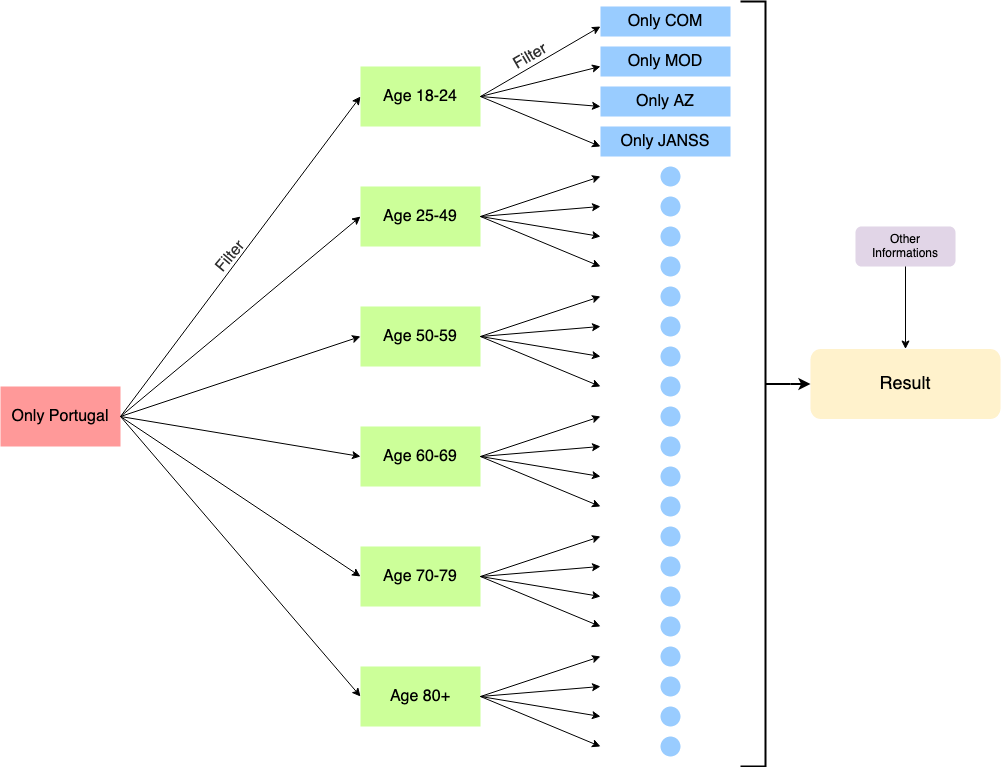
\includegraphics[width=300pt,trim=10 0 0 -10mm]{images/coiso2.png}
\caption{Data processing overview}
\label{fig:overview2}
\end{figure}

The \verb!Result! that we see in this figure, it's a reactive value with the data frame that will be used to render the plot.\\ This scheme, it's very similar in all data processing.\\

To render this plot, we use the \texttt{renderPlot()} function and save the result on a variable that will be the output displayed in the application. This behavior it's the same in all plots that we will show.\\
In this case, we call the data frame created at the end of the data processing, and we use the \texttt{ggplot()} function to create the plot. Then, as we want to display our plot in bars, with some visible information, we use the \texttt{geom\_bar()} and \texttt{geom\_text()} functions. We have some attributes in the \texttt{ggplot()} function that lets us handle with some theme and aesthetic details.
\\ To be easier to understand, consider this:
\begin{itemize}
    \item The 'Result' data frame will have the following structure:
    \begin{center}
        \begin{tabular}{ |c|c|c| } 
             \hline
             \textbf{{Idade}} & \textbf{Vac} & \textbf{Doses} \\ \hline
             Age group & Name of Laboratory/Vaccine & Number of people vaccinated \\  
             ... & ... & ...\\
             \hline
        \end{tabular}
    \end{center}
\end{itemize} 

Next we will show the actual code to render the plot that we want:\\

\begin{verbatim}
    output$myPlotPais <- renderPlot({
  
  res <- myReactiveDataPais() # Save the data set in the variable 'res'
  ggplot(res, aes(x= Vac, y=Doses, fill = Idades)) + 
    geom_bar(stat='identity', position = position_dodge())+
    geom_text(aes(label = Doses), vjust = -0.2,
              position = position_dodge(0.9), size = 3) +
    theme(
      axis.text.x = element_text(vjust = 1, size = 10,),
      axis.text.y = element_blank(),
      axis.ticks.y = element_blank(),
      axis.title = element_text(face="bold", size=18),
      title = element_text(size = 20),
      panel.grid = element_blank(),
      panel.background = element_rect(fill ="#ffffff")
    ) + 
    guides(fill= guide_legend(title = "Faixas etárias:")) +
    xlab('') + 
    ylab('') 
  
})
\end{verbatim}

As you can see, this is a good example to show how we render plots, after the data processing. In the future, this example will not be displayed here again. \\
The result of this plot  (\ref{fig:ages-vac}) is the following:\\

\begin{figure}[H]
\centering
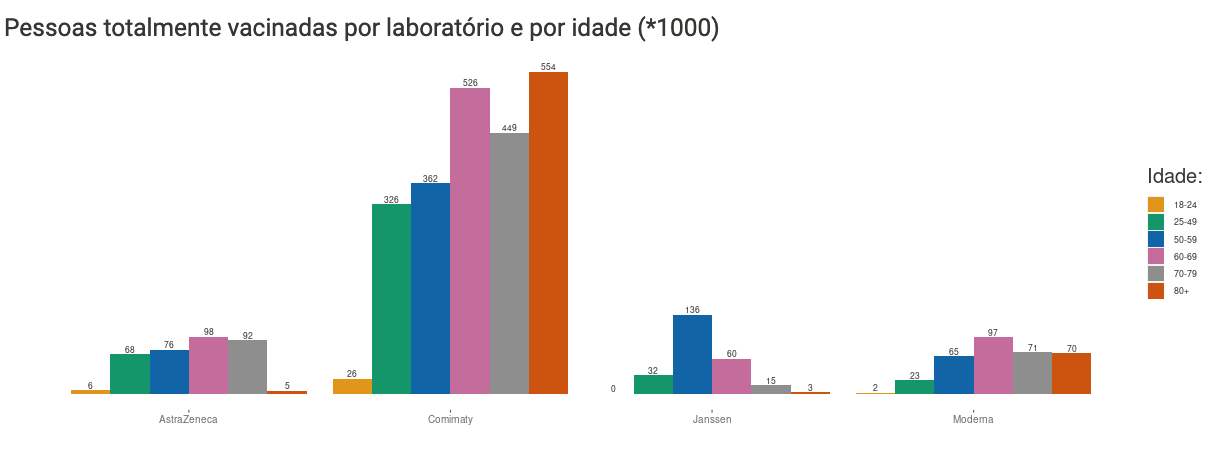
\includegraphics[width=400pt,trim=10 0 0 -10mm]{images/coiso3.png}
\caption{Plot of people totally vaccinated by age and laboratory}
\label{fig:ages-vac}
\end{figure}


\subsubsection{People totally vaccinated by age, by week}
This is a time plot segmented by age,  to visualise the behaviour of the number of vaccinated people,  week by week, in each group age.\\
Since there are much information in this graphic, we choose to give the user options to see the data.\\
The user can choose if he wants to see, or not, the value in each age group by week. %It's possible to choose how many age groups want  display simultaneously in the plot. This makes it possible for the user to compare as many as he wants.\\
\\
It is possible to choose how many age groups you want to display simultaneously on the chart. This allows the user to compare those vaccinated according to age.
\\
As mention earlier, the data processing it's pretty much similar, and this is one of those cases. Such as the previous graphic, we will filter the data set that have information only from Portugal, creating new data sets with specific information that we need to move on. In each one of these data sets, we need to preserve the week of vaccination and, for each week, sum all the people vaccinated by age group.
After the data processing, the result should be something with this structure:\\

    \begin{center}
        \begin{tabular}{ |c|c|c|c|c| } 
             \hline
             \textbf{\textit{Datas}} & \textbf{\textit{Vacinados18\_24}} & \textbf{\textit{Vacinados25\_49}} & \textbf{\textit{Vacinados\_ageGroup}} & ...\\ \hline
             Week$_n$ & \texttt{int} & \texttt{int} & \texttt{int} & ... \\  
             \hline
             Week$_{n+1}$ & \texttt{int} & \texttt{int} & \texttt{int} & ... \\  
             \hline 
             ... & ... & ... & ... & ...\\
             \hline
        \end{tabular}
    \end{center}

To render this plot, the process is the same as the previous plot, except that, in this one, we'll save the \texttt{ggplot()} in a variable (this is a feature of the graphics produced with \verb!ggplot2!). This makes possible that, in the future, we can add more information to this plot.\\
This information it's input passed by the user. When he chooses some option, our plot will update, adding or removing the information that he chose. Next we'll show different ways to observe the plot (\ref{fig:ages-vac-1})

\begin{figure}[H]
\centering
%width=\textwidth
%width=350pt,trim=10 0 0 -10mm
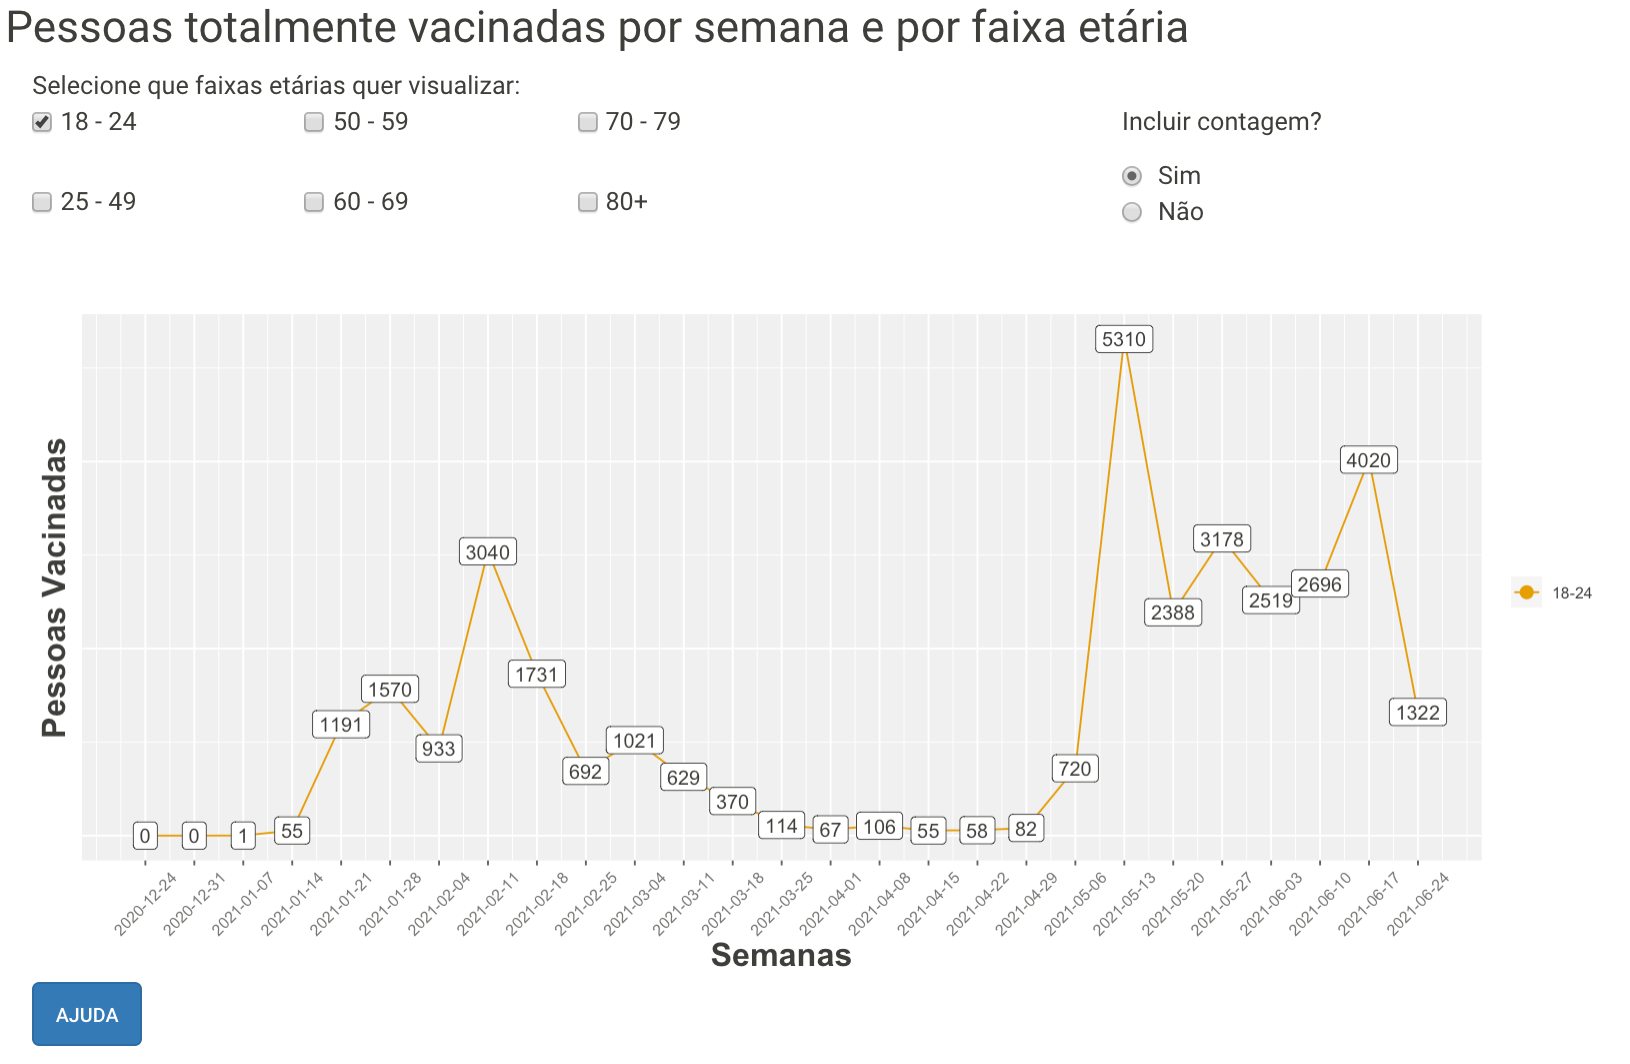
\includegraphics[width=\textwidth]{images/p1.png}
\caption{Plot with count, of the age group 18-24}
\label{fig:ages-vac-1}
\end{figure}
 As you can see, in the graphic (\ref{fig:ages-vac-1}), we include count and the age group selected is only 18-24.\\

\begin{figure}[H]
\centering
%width=350pt,trim=10 0 0 -10mm
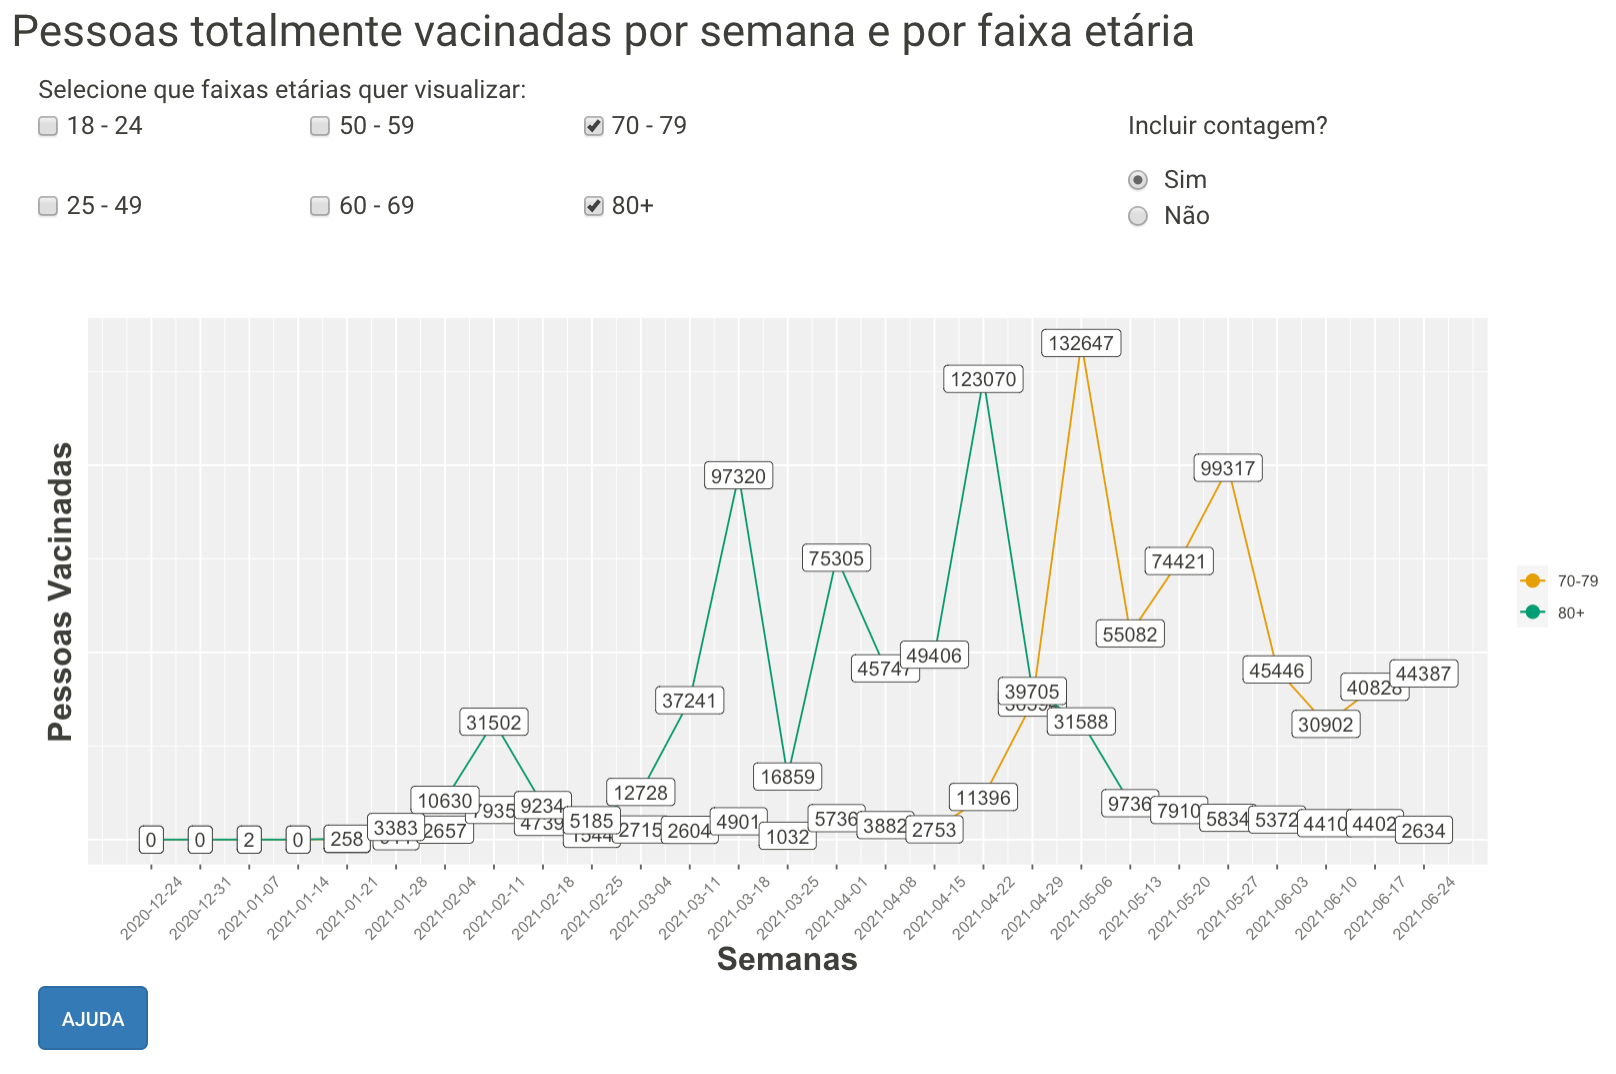
\includegraphics[width=\textwidth]{images/p2.png}
\caption{Plot with count, of the age groups 70-79 and 80+}
\label{fig:ages-vac-3}
\end{figure}
In the graphic (\ref{fig:ages-vac-3}), we include count and the age groups selected are 70-79 and 80+. This makes possible for the user to compare information.\\
As you can see, if you want to have an intuitive view of the evolution in every week, with the values displayed turns out to be hard.\\
That's the reason to give the option without the count. As shown next, Figure \ref{fig:ages-vac-4},  it's possible even to see some information justified by the vaccination plane and more. 

\begin{figure}[H]
\centering
%width=350pt,trim=10 0 0 -10mm
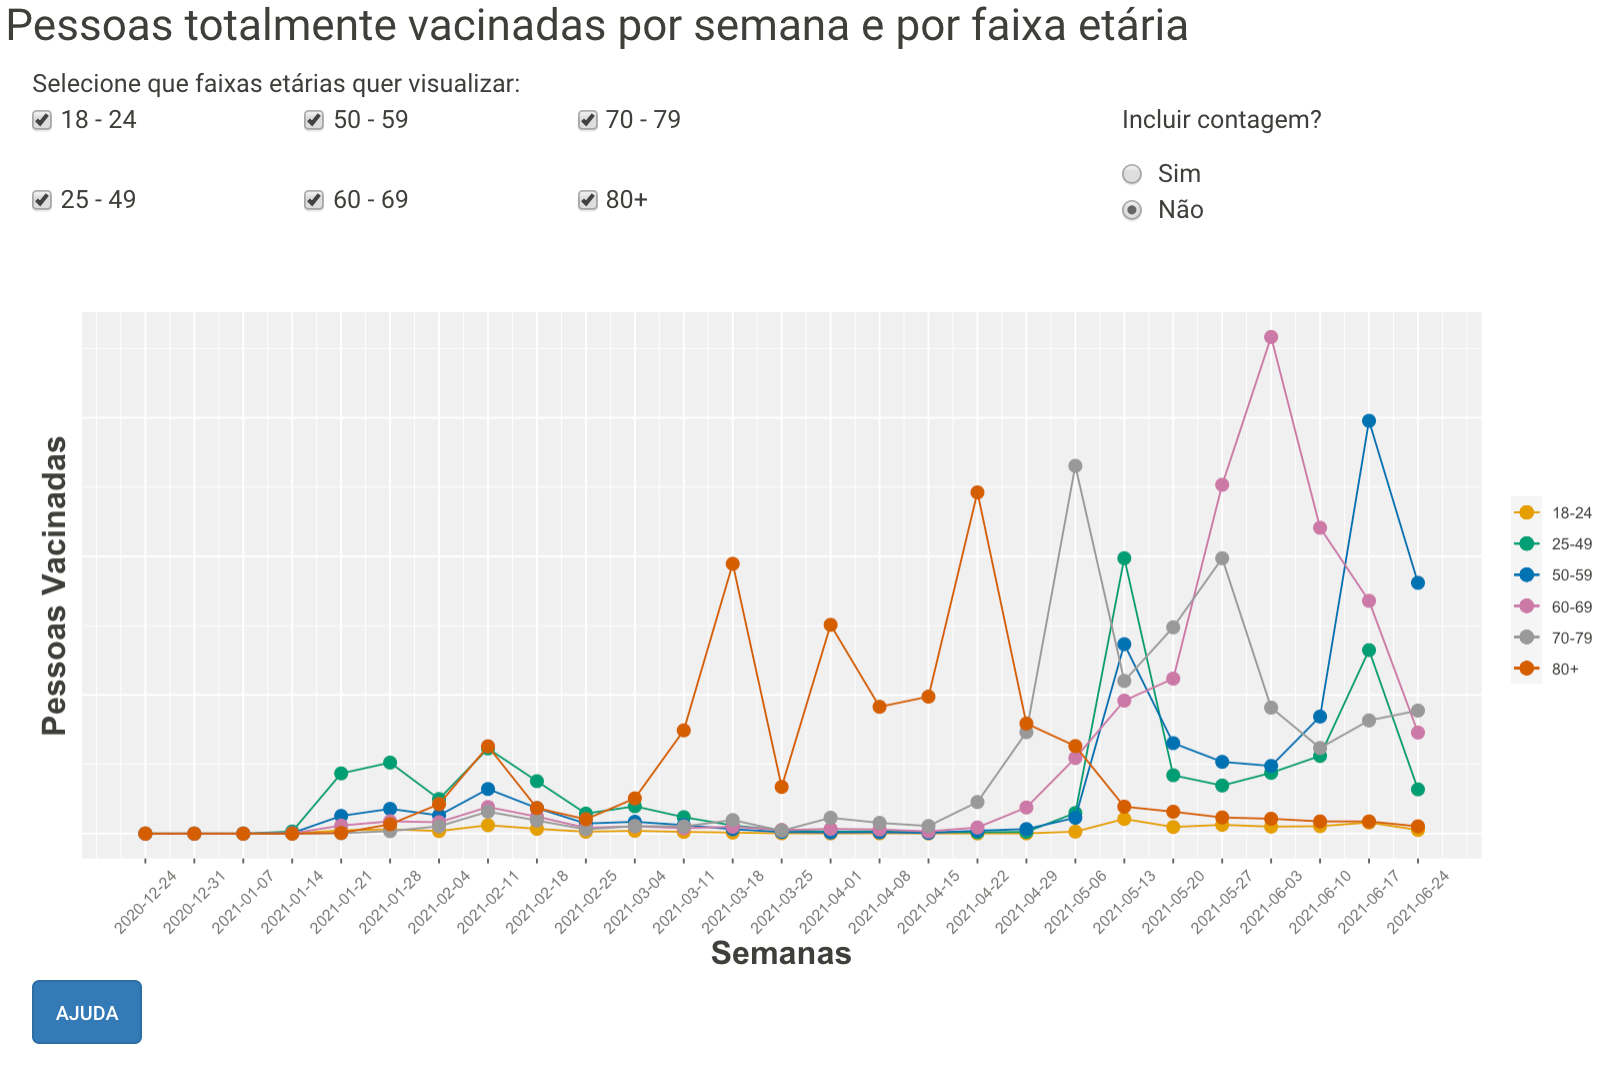
\includegraphics[width=\textwidth]{images/p4.png}
\caption{Plot without count, of all age groups}
\label{fig:ages-vac-4}
\end{figure}

\subsubsection{People totally vaccinated by region, by week}

This one it's exactly the same as the one before, with the difference of filter the total of people vaccinated by region, instead of group age.

\subsubsection{Vaccines administered by laboratory}

In terms of data processing, there's not any new way to do things. The result will be the shown in (\ref{fig:ages-vac-5}).\\
\begin{figure}[H]
\centering
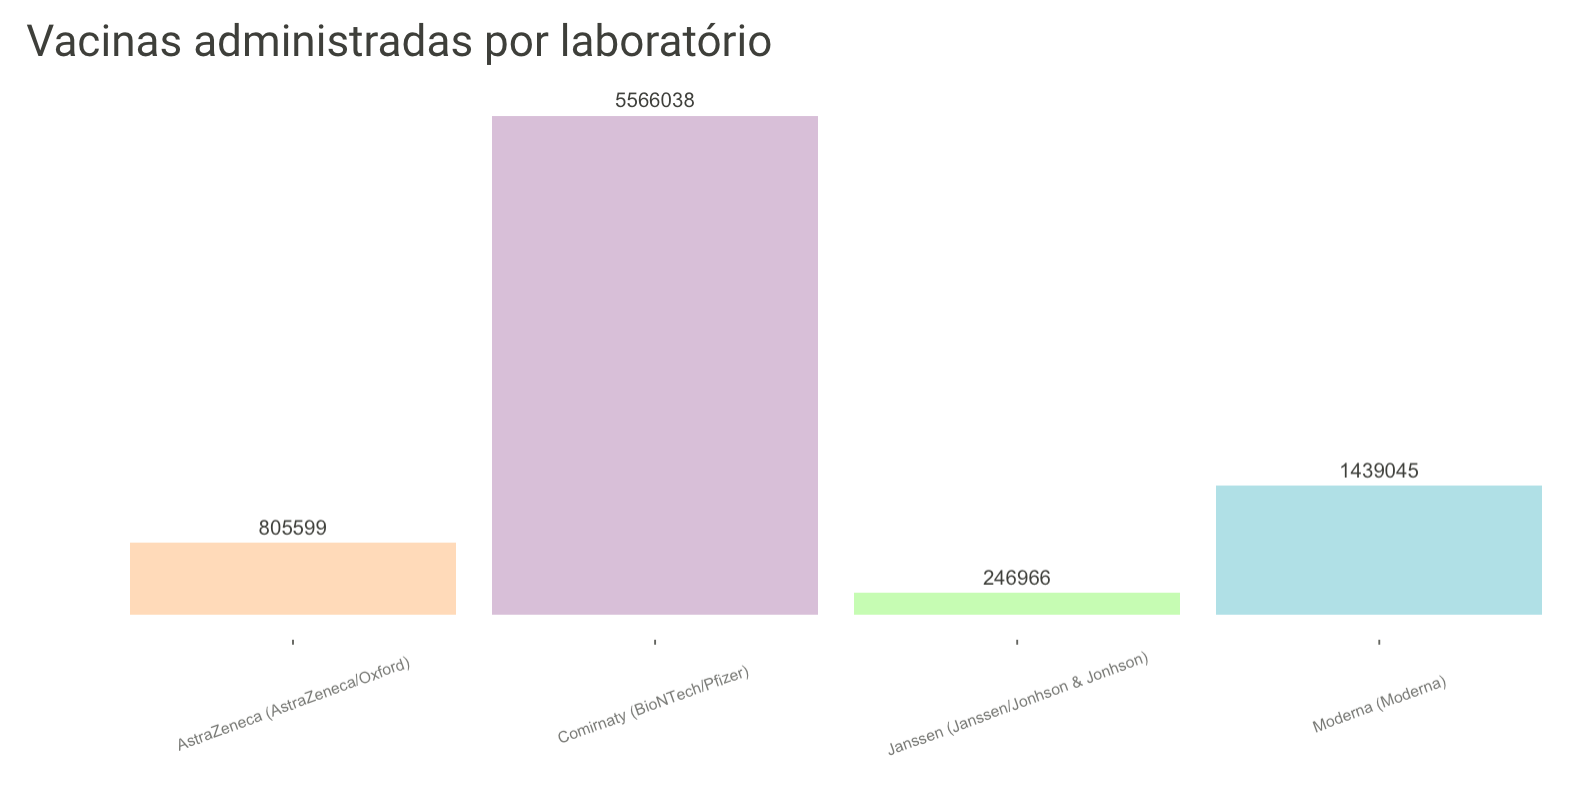
\includegraphics[width=350pt,trim=10 0 0 -10mm]{images/p5.png}
\caption{Plot with the number of administered vaccines by laboratory}
\label{fig:ages-vac-5}
\end{figure}

In this plot, all the administered doses are referent of the first and second dose of each vaccine.

\subsubsection{Percentages of vaccinated and unvaccinated people}

In this graphic, the data process is similar to the previous graphics with the exception that now, we want to work with percentages. With this in mind, we know the population of Portugal and with simple math it's easy to create the reactive value to render the plot.\\
\\
This graphic (\ref{fig:ages-vac-6}) uses a function from another package ('waffle'), that allow the function \texttt{renderPlot()} to display the information in a waffle plot. 
\begin{figure}[H]
\centering
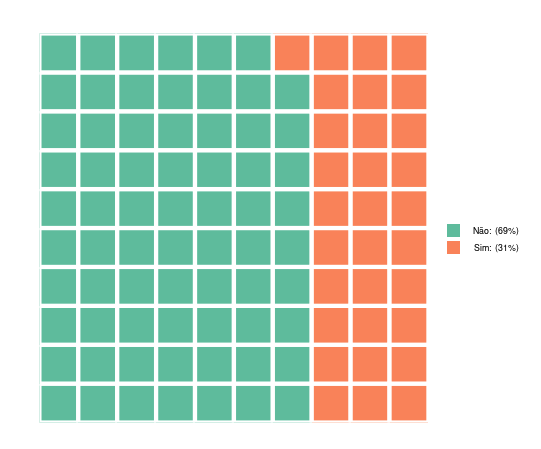
\includegraphics[width=200pt,trim=10 0 0 -10mm]{images/p6.png}
\caption{Plot with the percentages of vaccinated/unvaccinated people}
\label{fig:ages-vac-6}
\end{figure}
We choose to develop this plot this way, not only because, in our opinion, it looks good, but also to show that \textbf{ggplot2} can be very versatile.

\subsection{Regions}

First of all we began by filtering our dataset as soon as the App begins to load so that further ahead when we need the data for the selected region it's already filtered. For this purpose we used the \verb!reactiveVal()! function to create eight {\sf{reactive value}} objects. One for each region and another one for the whole country. The package used for this endeavour was the \verb!dplyr! package and was used as follows:
\begin{itemize}
\item We begin by creating the reactive object:

\begin{verbatim}
loaded_Alentejo <- reactiveVal()
\end{verbatim}

\item And end by loading it with the filtered data:

\begin{verbatim}
Alentejo <- loadedData2() %>% filter(Region == "PTCSR01")
loaded_Alentejo(Alentejo)
\end{verbatim}

Where \verb!loadedData2()! is the data for the whole country.
\end{itemize}
Having done this and in order to know the selected region tab, we gave an id to the Regions tab upon drawing our User Interface so that at the point of which we started to manipulate our data we would know the region we were dealing with. 

\subsubsection{Administered vaccines by week}

We begin by clearing the dataset of the unnecessary columns for the graphic. After this we are left with four columns: \verb!YearWeekIS0!, \verb!FirstDose!,
\\
\verb!SecondDose! and \verb!Vaccine!. 
\\
Having done this we'll need to add the doses of every vaccine available in each and every week and place all those values in an array. What we mean by this is: If a week has 4 reports, each relative to a certain type of vaccine, we'll need to add every First and Second Dose of all those four types and associate that sum to the week.
Finally we create a data-set with the Dates and with the Doses, and since we are taking care of this data with the reactive function, when we call such function in the renderPlot we'll receive the data-set.

In the renderPlot function all we'll have to do is give the ggplot function, from the ggpplot2 package, the data-frame, the aesthetic mappings of the contents of the data-frame, and add geom\_bar() with stat='identity' so that ggplot2 knows that we'll provide the y values. Here's an example on how that would look like:

\begin{verbatim}
output$yourPlotID <- renderPlot({

  res <- myReactiveDat()      ## the data-frame

  ggplot(res, aes(x=Data, y= Doses,fill=Doses)) +  
    geom_bar(stat='identity')+ 
    scale_fill_gradient(low="#63ACAA",high="#507D94")+          ##visual settings
    theme(axis.text.x = element_text(angle = 45, vjust = 0.5), 
          axis.title = element_text(face="bold", size=18),
          title = element_text(size = 20)) + 
    xlab('Week') +
    ylab('Doses')
})
\end{verbatim}

Here's how this graphic would look like (\ref{fig:diagrama}):

\begin{figure}[H]
\centering
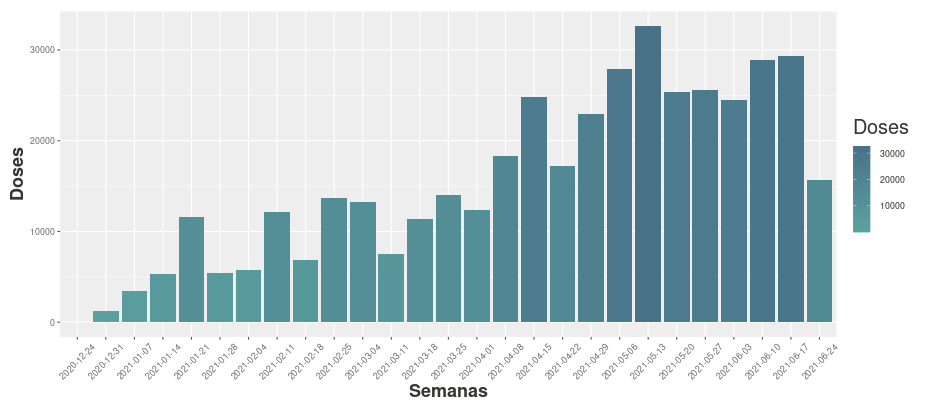
\includegraphics[width=300pt,trim=10 0 0 -10mm]{images/grafico1novo.png}
\caption{Administered vaccines by week}
\label{fig:diagrama}
\end{figure}

\subsubsection{Cumulative value of vaccines by week}

This graphic will follow the exact same principle of the previous one, however, this time we'll have to apply the "cumsum" function from RStudio to our Doses vector. This function returns a vector whose elements are the cumulative sums of the elements of the argument and was used as follows:

\begin{verbatim}
output$yourPlotID <- renderPlot({
  
  res <- myReactiveDat()
  
  (ggplot(res, aes(x=Data, y=cumsum(Doses),group=1))
    + geom_line(color="#63ACAA")
    + geom_point(color="#507D94") 
    + theme(axis.text.x = element_text(angle = 45, vjust = 0.5),
            axis.title = element_text(face="bold", size=18),
            title = element_text(size = 20))  
    + xlab('Week') 
    + ylab('Doses')
    
  )
})
\end{verbatim}

As you can see, the data used is the same as the one in the first graphic, except for the fact that we'll apply the function to the 'Doses' vector.
And since we're trying to see the progress we use the geom\_line function as well as the geom\_point function for a better perception of the results.


Here's how this graphic would look like (\ref{fig:diagrama1})
\begin{figure}[H]
\centering
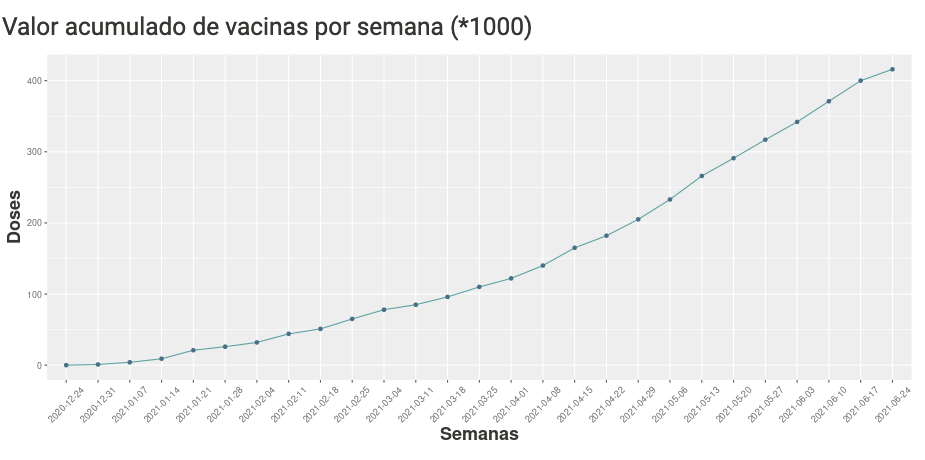
\includegraphics[width=300pt,trim=10 0 0 -10mm]{images/grafico2novo.png}
\caption{Cumulative value of vaccines by week}
\label{fig:diagrama1}
\end{figure}

\subsubsection{Percentage: Vaccinated/Incomplete Vaccination}

For this chart we had to pay careful attention to the data for each region since there are certain Vaccine brands that are yet to be administered in some regions. Having this in consideration and the vaccination treatment of each vaccine, the procedure to find the intended values to draw the waffle chart will consist in getting the sum of all the Second Doses from Moderna, Pfizer and AstraZeneca vaccines and adding the sum of all the First Doses of the Jansen vaccine. This total will be the amount of people that are completely vaccinated and if we subtract it from the population of the region we'll get the amount of people that haven't completed the full vaccination treatment.

After getting both values, in order to get the percentages, all we had to do was dividing both numbers by the region population and multiplying the result by 100. Then we create a vector with both percentages and since we're working on this data with the reactive function, when we call it we'll receive said vector.

Finally we draw our Waffle chart (\ref{fig:diagrama2})
\begin{verbatim}
output$yourPlotID <- renderPlot({
  resWaffle <- myReactiveWaffles()
  val_names <- sprintf("%s (%s%%)", 
                       c("Vacinação incompleta: ", 
                         "Completamente Vacinados: "), 
                       resPie)
  names(resWaffle) <- val_names
  waffle::waffle(resPie)
})
\end{verbatim}

\begin{figure}[H]
\centering
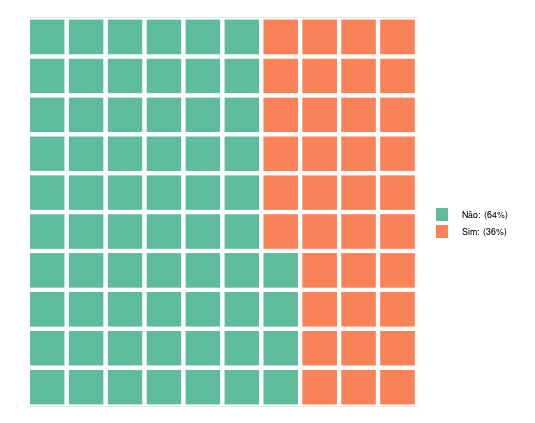
\includegraphics[width=300pt,trim=10 0 0 -10mm]{images/graficomapa2.png}
\caption{Percentage: Vaccinated/Incomplete Vaccination}
\label{fig:diagrama2}
\end{figure}

\subsubsection{Administered vaccines by laboratory}

We start off by filtering the data for every vaccine. After this we'll need to verify whether the data frame of each vaccine is not empty just in case the region we're dealing with has not received any vaccines of that laboratory. If the data frames are not empty, we'll create a variable for each one with the sum of both the First Doses as well as the Second Doses. At last a vector with these values is created so that, when we call the reactive function in the renderPlot, we can access this data.

Here's how the renderPlot function would look like:

\begin{verbatim}
output$yourPlotID <- renderPlot({
  
  res <- VacinasReg()
  ggplot(res, aes(x=Nomes, y=Totais, fill = c6)) + 
    geom_bar(stat='identity')+ 
    scale_fill_manual(values = c("AZ"="#D8BFD8",
                                 "MOD"="#B0E0E6",
                                 "COM"="#FFDAB9",
                                 "JJ"="#c6ffb3")) +
    geom_text(aes(label=Totais), vjust = -0.6, size = 4)+
    theme(
      legend.position = "none",
      axis.text.x = element_text(angle = 20, vjust = 0.5),
      axis.title = element_text(face="bold", size=18),
      axis.text.y = element_blank(),
      axis.ticks.y = element_blank(),
      title = element_text(vjust = 1, size = 20),
      panel.grid = element_blank(),
      panel.background = element_rect(fill ="#ffffff")
    ) + 
    xlab('') +
    ylab('') 
})
\end{verbatim}

As we can see, the res variable will consist of a data frame with both the names of the vaccines as well as the totals. Knowing this, the process to draw the graphic is more or less the same as most of the others. We pass these values onto the ggplot function and after that we add the geom\_bar in order to draw an bar plot (\ref{fig:diagrama3}). 

\begin{figure}[H]
\centering
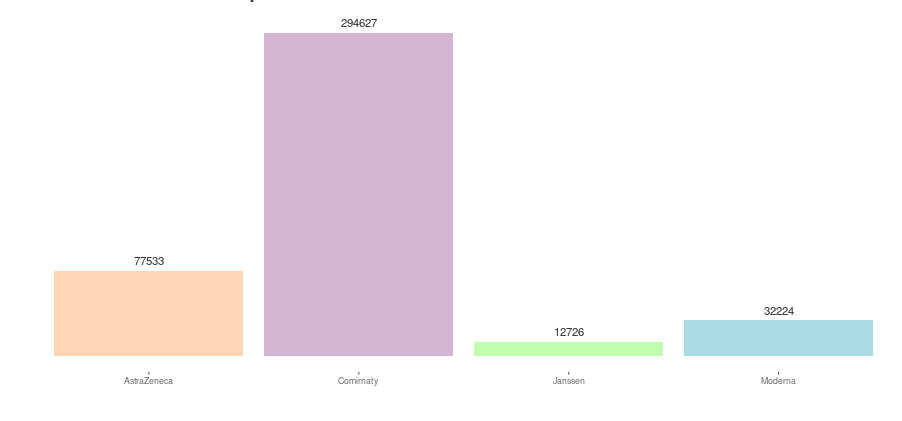
\includegraphics[width=300pt,trim=10 0 0 -10mm]{images/grafico4novo.png}
\caption{Administered vaccines by laboratory}
\label{fig:diagrama3}
\end{figure}

\section{Publication}
It's possible to public the application for free, on the internet using \url{https://www.shinyapps.io}. \cite{io} This is an online service for hosting Shiny apps in the cloud. RStudio takes care of all the details of hosting the app and maintaining the server.
We found out pretty simple to publish the application. It's just creating an account and follow the well described steps. It tokes us a bit of time because we had to correct some errors that prevented publication correctly, but an experiment developer should do this steps quicker. Our application is located in the following link:\\
\\
\href{https://rafaelantunes.shinyapps.io/VacinacaoPortugal/}{https://rafaelantunes.shinyapps.io/VacinacaoPortugal/}

\chapter{Conclusion}

This project made us realize the versatility of the Shiny package from RStudio. We were baffled by how easy it was to build a very useful app with such little tools. Even though we added a bit of HTML and CSS ourselves it was clear that someone with very little knowledge of front-end development and some R language knowledge could very well develop an interesting app.

\bibliographystyle{plain}
\begin{thebibliography}{10}

\bibitem{R-project website} \url{https://www.r-project.org/about.html}, \textbf{About R-Project website}
\bibitem{RStudio}, \textbf{ RStudio website} \url{https://www.rstudio.com}
\bibitem{shiny}\url{https://shiny.rstudio.com/l}{https://shiny.rstudio.com}, \textbf{Shiny website}
\bibitem{SARS-CoV-2}\url{https://apps.who.int/iris/bitstream/handle/10665/332197/WHO-2019-nCoV-FAQ-Virus_origin-2020.1-eng.pdf},\textbf{ Origin of SARS-CoV-2 - \ac{WHO}}
\bibitem{wiki} \url{https://en.wikipedia.org/wiki/COVID-19_pandemic} \textbf{About COVID-19 pandemic -- wikipedia}
\bibitem{EU}\url{https://ec.europa.eu/info/live-work-travel-eu/coronavirus-response/public-health/eu-vaccines-strategy_pt}, \textbf{EU vaccine strategy} 
\bibitem{owd}\url{https://ourworldindata.org}
\bibitem{reuters}\url{https://graphics.reuters.com/world-coronavirus-tracker-and-maps/vaccination-rollout-and-access/}, \textbf{Covid-19 vaccination tracker, Reuters} 


\bibitem{pubINE}\url{https://www.ine.pt/xurl/pub/71882686}, \textbf{Instituto Nacional de Estatística - Estatísticas Demográficas : 2019. Lisboa : INE, 2020.} 


\bibitem{trab}\url{https://ec.europa.eu/eures/main.jsp?acro=lmi&lang=pt&countryId=PT&catId=57&parentId=0}, \textbf{Labor Market Information - European Commission} 

\bibitem{dataDownload}\url{https://vaccinetracker.ecdc.europa.eu/public/extensions/COVID-19/vaccine-tracker.html#uptake-tab}, \textbf{General Vaccine information - European Centre for Disease Prevention and Control } 

\bibitem{tidy}\url{https://vita.had.co.nz/papers/tidy-data.pdf}  \textbf{Tidy Data} 
\end{thebibliography}

\end{document}


